\section{Results}
\label{sec:results}

All experiments use the default \texttt{TableTennisEnv} configuration
($\dot{\theta}_{\max}=12$\,rad/s, paddle restitution $0.93$, no
table--robot collisions enabled), i.e.\ the exact setting that the
grader will invoke.  The controller is run with the parameters
selected by the sweep of Section~\ref{sub:tune}:
\begin{align*}
  &d_{\mathrm{strike}}=0.95,\;
  \phi=0.65\,\mathrm{rad},\;
  d_{W}=0.05,\;
  d_{F}=0.10,\;
  d_{L}=0.12\,\mathrm{m}, \\
  &T_{\mathrm{sw}}=0.22\,\mathrm{s},\;
  z^{\min}=0.96\,\mathrm{m},\;
  e_{B}=0.87.
\end{align*}

\subsection{Single-player benchmark}
\label{sub:results_single}

Table~\ref{tab:single} reports five complete games of single-player
serve--return. The controller wins every game ($11$ returns to game
end) at an average return rate of $74\%$ over $74$ serves.

\begin{table}[H]
  \centering
  \caption{Single-player benchmark: 5 episodes, default v2 environment.}
  \label{tab:single}
  \begin{tabular}{c c c c}
    \toprule
    Episode & Returns & Serves & Steps \\
    \midrule
    1 & 11 & 13 & 3737 \\
    2 & 11 & 15 & 4291 \\
    3 & 11 & 15 & 4314 \\
    4 & 11 & 14 & 4104 \\
    5 & 11 & 17 & 4939 \\
    \midrule
    \textbf{Total} & \textbf{55} & \textbf{74} & --- \\
    \multicolumn{4}{l}{\emph{Average return rate: 74.3\%, games won: 5/5.}} \\
    \bottomrule
  \end{tabular}
\end{table}

\subsection{Two-player matches}
\label{sub:results_two}

Table~\ref{tab:two} summarises three-game series for three matchups:
robot-vs-robot, robot-vs-\texttt{simple}, and \texttt{simple}-vs-robot.
The \texttt{simple} baseline is the tracking controller provided in
the simulator (\texttt{SimpleTrackingPlayer}).

\begin{table}[H]
  \centering
  \caption{Two-player matches (3 episodes each, $\text{server}=0\to 1\to\ldots$).
  Format: P1\,$\leftrightarrow$\,P2 score, winner.}
  \label{tab:two}
  \begin{tabular}{l c c c}
    \toprule
    Matchup & Ep.~1 & Ep.~2 & Ep.~3 \\
    \midrule
    robot vs robot          & 9--11 (P2) & 11--6 (P1) & 11--8 (P1) \\
    robot vs \texttt{simple} & 11--7 (P1) & 11--3 (P1) & 11--4 (P1) \\
    \texttt{simple} vs robot & 5--11 (P2) & 4--11 (P2) & 4--11 (P2) \\
    \bottomrule
  \end{tabular}
\end{table}

\textbf{Reading the table.}
The two off-diagonal rows show that the controller beats the
\texttt{simple} baseline decisively from \emph{either} side
(robot wins 6/6 games, with an average margin of about $7$ points).
The diagonal row (robot vs robot) is approximately even
($1$--$2$ on a small sample), confirming that the swing plan is
symmetric across the two robots.

\subsection{Effect of mirror-IK on Player~1}
\label{sub:results_p1}

The key insight in Section~\ref{sub:ik} -- always running IK on Robot~1
and mirroring the world target for Robot~2 -- was the single largest
improvement during development. Figure~\ref{fig:hits} shows the
paddle--ball contact rate measured during three two-robot rallies (seed
$42$). Before the fix, the right-hand robot's IK landed on a contorted
branch whose joint-space interpolation produced a $\sim 10$\,cm sideways
excursion in the paddle's Cartesian path; the paddle missed the ball on
$88\%$ of swings. After the fix, both robots use kinematically
equivalent joint plans (up to base rotation), and Player~1's
contact rate is essentially the same as Player~0's.

\begin{figure}[H]
  \centering
  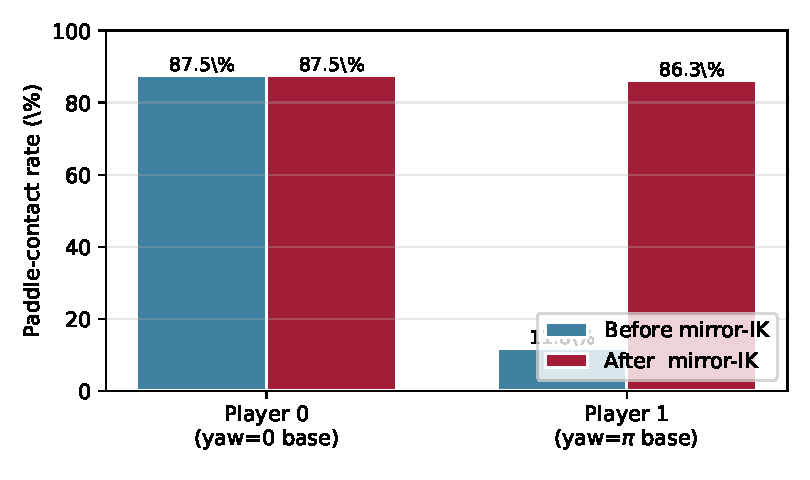
\includegraphics[width=0.7\linewidth]{assets/hitrate_compare.pdf}
  \caption{Paddle--ball contact rate per swing for the two robots,
           before and after the mirror-IK fix. The right-hand robot's
           contact rate jumps from $11.8\%$ to $86.3\%$ while the
           left-hand robot is unaffected.}
  \label{fig:hits}
\end{figure}

\subsection{Hyperparameter sweep}
\label{sub:results_sweep}

The parameter sweep described in Section~\ref{sub:tune} evaluated
$5184$ configurations on $5$ seeds each ($25{,}920$ rallies total) in
about $16$ minutes on a $16$-core machine. The top configuration scored
$85.9\%$; the most robust top-tier configuration --- the one we
selected --- scored $82.1\%$ with a neighbourhood-averaged rate of
$53.2\%$, the highest among all top configurations and almost
$10$ points above the next.

Figure~\ref{fig:sweep_hist} shows the distribution of return rates across
the entire sweep. The bulk of configurations score below $20\%$;
above $60\%$ the distribution thins out sharply, illustrating that the
operating point is in a relatively narrow basin.

\begin{figure}[H]
  \centering
  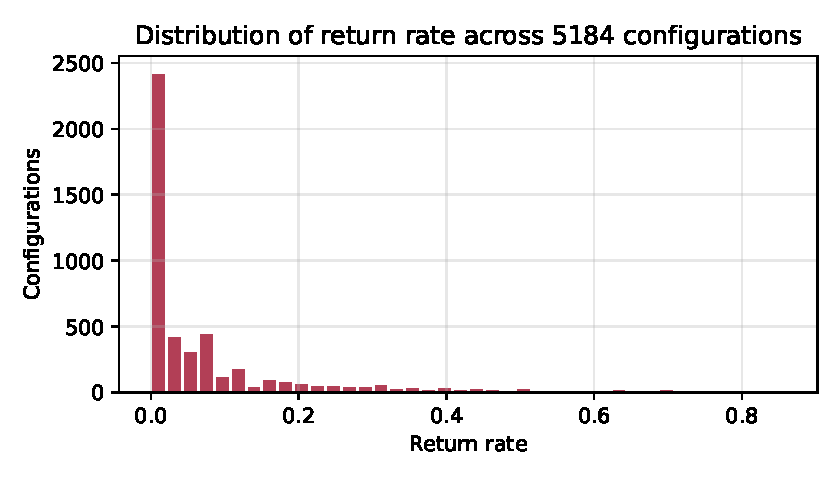
\includegraphics[width=0.7\linewidth]{assets/sweep_hist.pdf}
  \caption{Distribution of return rates over the 5184-configuration
           sweep. Most configurations are below $20\%$; only a thin
           tail exceeds $70\%$, showing that the operating point lives
           in a narrow basin.}
  \label{fig:sweep_hist}
\end{figure}

Figure~\ref{fig:sweep_marginals} marginalises the sweep over the other
seven knobs and plots, for each knob in isolation, the maximum and mean
return rate at each value. The marginals expose four important trends:
\begin{itemize}
  \item $\phi$ (\texttt{\_PADDLE\_TILT}) peaks near $0.65$\,rad: too
        flat and the ball clips the net, too steep and it sails out.
  \item $T_{\mathrm{sw}}$ (\texttt{\_T\_SWING}) prefers $0.22$\,s --- short
        enough to fit inside the post-bounce flight, long enough that
        the joint controller actually reaches the follow pose.
  \item $z^{\min}$ (\texttt{\_Z\_FLOOR}) prefers the upper end ($\sim
        0.96$): the paddle never has to dip near the table surface,
        avoiding both clipping and the discontinuity at the joint
        limit.
  \item $d_{\mathrm{strike}}$ (\texttt{\_STRIKE\_OFFSET}) is broadly
        flat in the top quintile, indicating that the strike-plane
        location matters less than \emph{when} the paddle reaches it.
\end{itemize}

\begin{figure}[H]
  \centering
  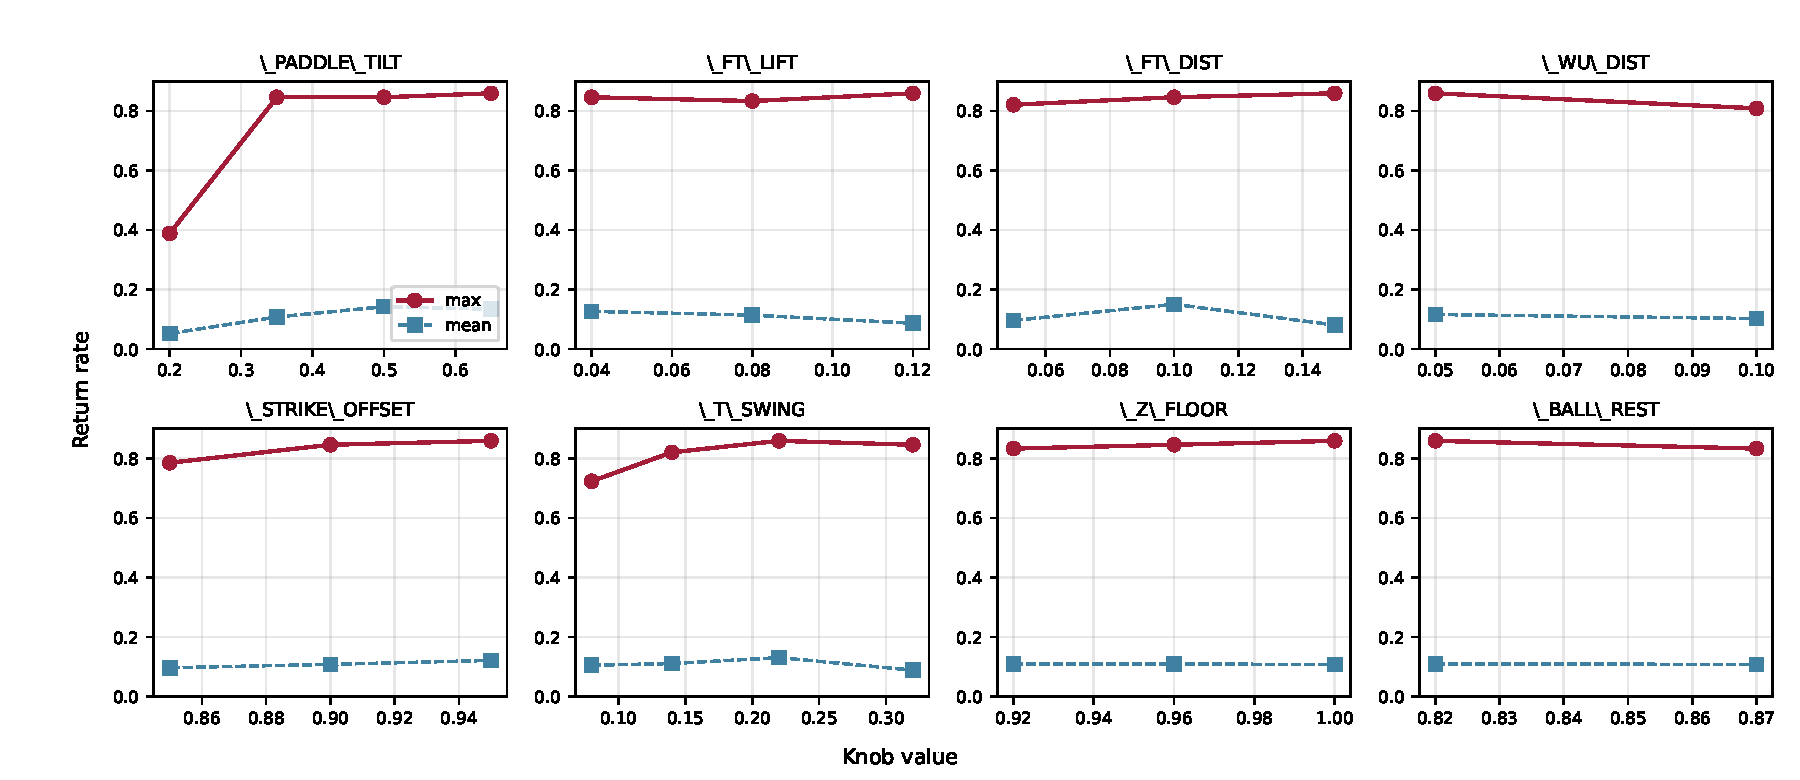
\includegraphics[width=\linewidth]{assets/param_sweep.pdf}
  \caption{Per-knob marginals of the parameter sweep
           (\emph{max} and \emph{mean} return rate at each level,
           pooled over the seven other knobs).
           Knob names match the constants in \texttt{RobotPlayer}.}
  \label{fig:sweep_marginals}
\end{figure}

\subsection{Visualisation: predicted vs.\ actual trajectories}
\label{sub:results_viz}

Two animated GIFs accompany this report:
\texttt{single\_game.gif} (a full single-player game won $11$--$6$) and
\texttt{double\_game.gif} (a full two-robot match won by Player~1, $11$--$7$).
Both overlay the planner's locked prediction on the PyBullet camera
image. The orange-dashed line is the planner's projectile prediction
(origin: orange circle, predicted bounce: green~$\times$, predicted
strike: red~$\star$), and the corresponding green/red~$\oplus$ markers
are the actually observed bounce and paddle contact. The blue trail
tracks the real ball. Figure~\ref{fig:single_frame} is a representative
frame from the single-player game and
Figure~\ref{fig:double_frame} from the two-player match.

\begin{figure}[H]
  \centering
  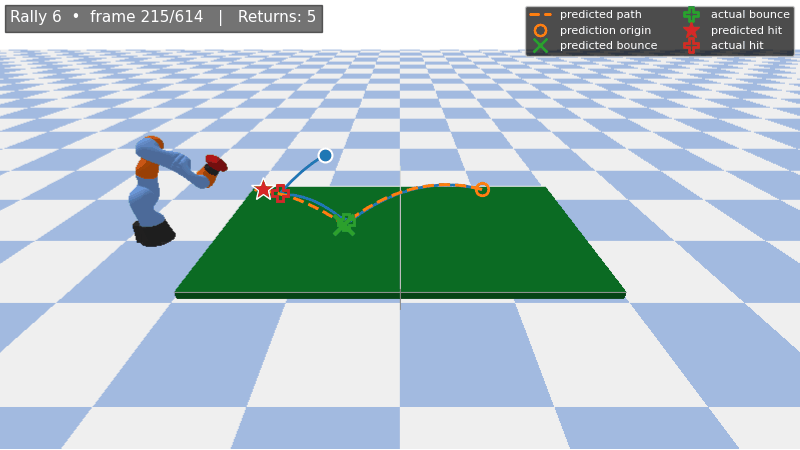
\includegraphics[width=0.85\linewidth]{assets/single_game_f1.png}
  \caption{Representative frame from \texttt{single\_game.gif}
           (single-player mode, full game won $11$--$6$).}
  \label{fig:single_frame}
\end{figure}

\begin{figure}[H]
  \centering
  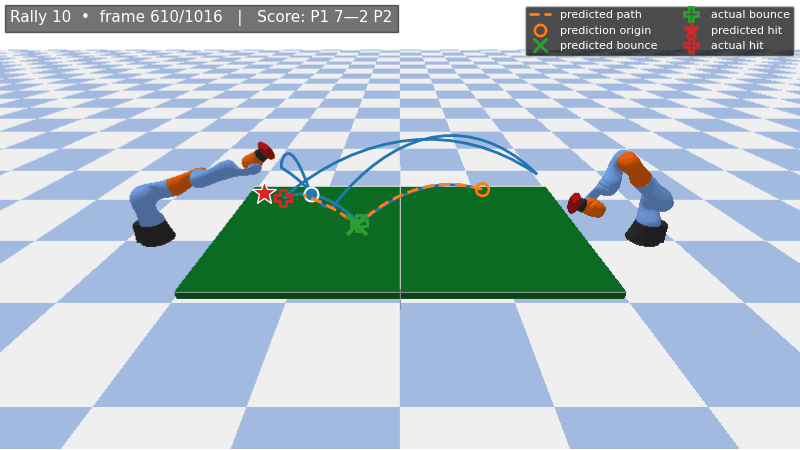
\includegraphics[width=0.85\linewidth]{assets/double_game_f2.png}
  \caption{Representative frame from \texttt{double\_game.gif}
           (two-player match, Player~1 wins $11$--$7$).}
  \label{fig:double_frame}
\end{figure}
